% document type
\documentclass[12pt]{article}

% packages
\usepackage[total={170mm,230mm}]{geometry}
\usepackage[utf8]{inputenc}
\usepackage[T1]{fontenc}
\usepackage[russian]{babel}
\usepackage{graphicx}
\usepackage{amssymb}
\usepackage{amsfonts}
\usepackage{amsmath}
\usepackage{amsthm}
\usepackage{physics}
\usepackage{nicefrac}
\usepackage{cancel}
\usepackage{hyperref}
\usepackage{cmap}

\title{Опыт Франка\---Герца}
\author{Козлов Александр \and Краснощёкова Дарья}

\begin{document}
	\maketitle
	\section{Определение резонансного потенциала}
	Сняли анодно\---сеточную характеристику при задерживающем напряжении, при котором видно два максимума анодно\---сеточной характеристики наилучшим образом. Задерживающее напряжение было выбрано $12.1 \pm 0.1\ \text{В}$. Результаты измерений отображены на рисунке \ref{fig:figure1}.
	\begin{figure}[htbp]
		\centering
		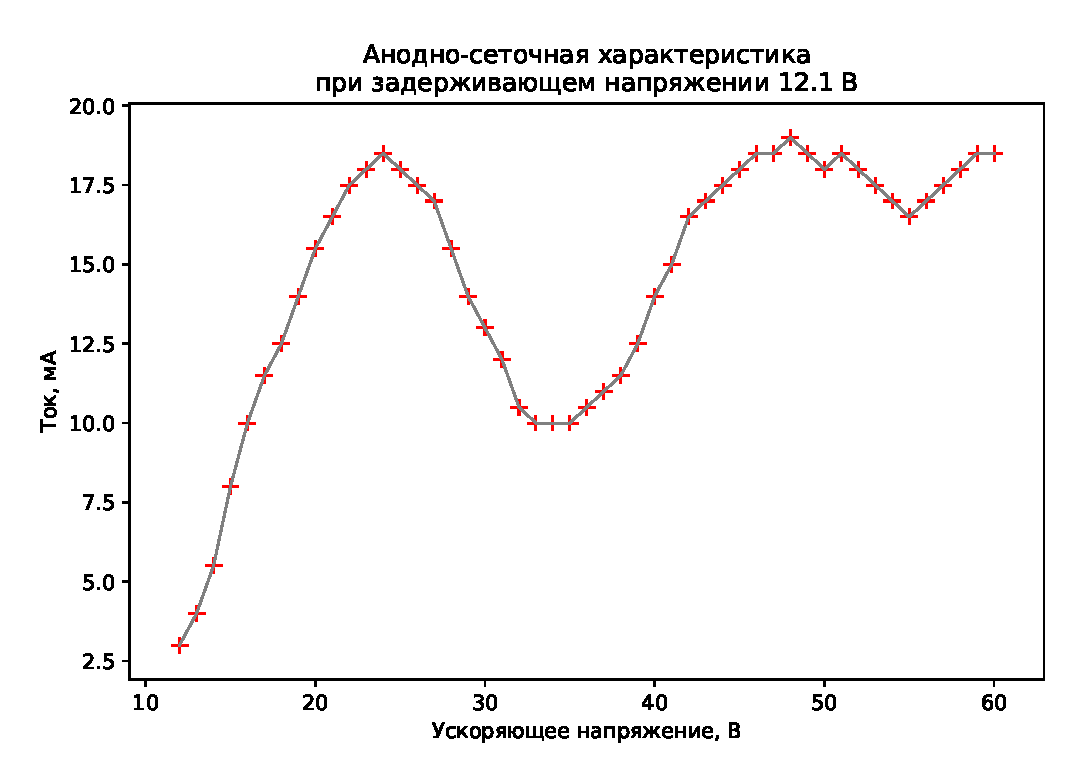
\includegraphics[width=\linewidth]{../plots/1}
		\caption{Анодно-сеточная характеристика при задерживающем напряжении $12.1\ \text{В}$.}
		\label{fig:figure1}
	\end{figure}
	Первые два локальных максимума обнаружены при ускоряющих потенциалах $\varphi_1=24.0\pm0.5\ \text{В}$ и $\varphi_1=48.0\pm0.5\ \text{В}$. Из наших измерений оказалось, что не важно каким именно образом определять резонансное напряжение. Можно как через напряжение первого локального максимума ($\varphi_1=24.0\pm0.5\ \text{В}$), так и через разность напряжений второго и первого локальных максимумов анодно\---сеточной характеристики ($\varphi_1 - \varphi_2 = 24\pm1\ \text{В}$). Таким образом, $V_\text{рез} = 24\pm0.5\ \text{В}$. Отсюда находим разность энергий
	\begin{equation}
			E_1 - E_0 = eV_\text{рез} = 24.0\pm0.5\ \text{эВ}.
	\end{equation}
	\par Стоит отметить, что резонансный потенцил гелия отличается от измеренного нами. В действительности он составляет $24\ \text{В}$.

	\section{Определение потенциала ионизации}
	
\end{document}